%% IEEE conference paper -- International Conference on Artificial Intelligence
%% and Emerging Technologies (ICAIET 2027), XIM University, Bhubaneswar, India.
%% Track: Machine Learning and Data Science.
%%
%% Compile: pdflatex paper && pdflatex paper   (figures/*.png required)
%% Requires the standard IEEEtran document class (texlive-publishers / CTAN).
\documentclass[conference]{IEEEtran}
\IEEEoverridecommandlockouts

\usepackage{cite}
\usepackage{amsmath,amssymb,amsfonts}
\usepackage{graphicx}
\usepackage{booktabs}
\usepackage{textcomp}
\usepackage{xcolor}
\usepackage{url}
\usepackage{siunitx}

\DeclareSIUnit{\knot}{kn}

\graphicspath{{figures/}}

\begin{document}

\title{Data-Driven Surrogate Modelling for Early-Stage Ship-Hull Resistance
Prediction and Multi-Objective Design Exploration in Naval Architecture}

\author{\IEEEauthorblockN{Author Name(s)}
\IEEEauthorblockA{School of Computer Science and Engineering \\
XIM University \\
Bhubaneswar, India \\
email@domain}
\thanks{Author and affiliation details are placeholders to be completed before
camera-ready submission. All code, data-generation scripts and trained-model
artefacts accompanying this paper are provided in the supplementary
repository to support reproducibility.}}

\maketitle

\begin{abstract}
Calm-water resistance and the associated propulsive power are the single most
consequential performance figures fixed during the earliest stage of ship
design, yet they are also the most expensive to evaluate: model-scale towing
tests and Reynolds-Averaged Navier--Stokes (RANS) computational fluid dynamics
(CFD) each cost hours to days per candidate hull, which throttles the number
of designs a naval architect can realistically explore. This paper develops
and benchmarks a machine-learning (ML) surrogate framework that predicts the
total resistance of displacement hulls directly from their principal
particulars, and then uses the trained surrogate to perform large-scale
multi-objective design exploration. Using a reproducible dataset of
\num{5232} hull--speed operating points generated by Latin Hypercube Sampling
of a five-dimensional design space and labelled with a transparent
semi-empirical resistance oracle (ITTC-1957 friction line, a fullness-dependent
form factor, and a Froude-number-dependent residuary component), we compare six
regressors spanning linear, instance-based, ensemble-tree, neural, and
Gaussian-process families. The best models attain a coefficient of
determination $R^{2}=0.999$ and a mean absolute percentage error (MAPE) below
\SI{2}{\percent} on held-out hulls, and remain within \num{0.001} in $R^{2}$
under five-fold cross-validation. Gradient boosting screens \num{17599}
feasible candidate hulls in \SI{122}{\milli\second}
($\sim\!\num{144000}$~designs\,s$^{-1}$, \SI{7}{\micro\second} per design),
recovering a resistance--capability Pareto front whose members agree with the
verification oracle to within \SI{3.9}{\percent} MAPE---an evaluation
throughput that is orders of magnitude beyond direct CFD. We situate the study
within the broader landscape of ML in naval architecture, ocean engineering,
and shipbuilding, and outline a roadmap connecting surrogate-based design to
uncertainty-aware active learning, structural health monitoring, and
production-quality inspection. The framework is directly relevant to the
International Maritime Organization's tightening energy-efficiency regulations,
where rapid, low-cost exploration of resistance-optimal hulls is a lever for
maritime decarbonisation.
\end{abstract}

\begin{IEEEkeywords}
machine learning, surrogate modelling, naval architecture, ship resistance,
hull-form optimisation, ocean engineering, Gaussian process, gradient boosting,
multi-objective design, maritime decarbonisation.
\end{IEEEkeywords}

\section{Introduction}

\IEEEPARstart{S}{hipping} moves roughly \SI{80}{\percent} of global trade by
volume and is responsible for close to \SI{3}{\percent} of anthropogenic
greenhouse-gas emissions~\cite{imo2020,eu2023}. The International Maritime
Organization's Energy Efficiency Design Index (EEDI) for new ships and the
Energy Efficiency Existing Ship Index (EEXI), together with the operational
Carbon Intensity Indicator (CII), have converted hydrodynamic efficiency from a
commercial preference into a regulatory obligation~\cite{imo2020}. Because the
calm-water resistance of a hull---and hence its installed power, fuel burn and
carbon intensity---is very largely committed during the first weeks of a design
spiral, the early-stage designer's ability to \emph{search} the hull-form space
quickly and cheaply is now a decisive factor in a vessel's lifetime emissions.

That search is throttled by the cost of the evaluation itself. High-fidelity
resistance prediction rests on two pillars: physical model testing in a towing
tank, and numerical simulation by Reynolds-Averaged Navier--Stokes (RANS)
computational fluid dynamics (CFD). A single tank campaign requires a machined
scale model and days of facility time; a single well-resolved steady RANS
resistance computation for a full hull consumes on the order of hours to a day
of multi-core wall-clock time~\cite{molland2011,stern2013}. Neither scales to
the $10^{4}$--$10^{5}$ candidate hulls that a global, multi-objective
optimisation over principal particulars and hull-form parameters would ideally
visit. In practice designers fall back on low-order empirical regressions such
as the Holtrop--Mennen method~\cite{holtrop1982} or on coarse design charts,
trading accuracy and generality for speed.

Machine learning offers a third path. A \emph{surrogate model}---a fast,
differentiable statistical approximation trained once on a corpus of
high-fidelity evaluations---can replace the expensive evaluator inside the
optimisation loop, returning a prediction in microseconds while retaining a
large fraction of the fidelity of the data it was trained on~\cite{forrester2008,
queipo2005}. Surrogate-based design and optimisation is now standard in
aerospace and automotive engineering, and a growing body of work applies it to
marine hydrodynamics~\cite{ao2021,cepowski2020,marlantes2023}. What is often
missing from that literature, however, is a controlled, end-to-end and
\emph{reproducible} comparison of modern regressor families on a common
resistance-prediction benchmark, coupled to a concrete demonstration of the
design-exploration throughput the surrogate unlocks.

\subsection*{Contributions}
This paper makes the following contributions.
\begin{enumerate}
\item \textbf{A reproducible resistance-surrogate benchmark.} We release a
transparent semi-empirical resistance oracle and a Latin-Hypercube-sampled
dataset of \num{5232} feasible displacement-hull operating points spanning a
realistic five-dimensional design envelope (length, beam, draft, block
coefficient, speed), together with the code that regenerates them from a fixed
seed.
\item \textbf{A head-to-head model study.} We benchmark six regressors---linear
regression, $k$-nearest-neighbours, random forest, gradient boosting, a
multilayer perceptron, and a Gaussian process---under a single protocol,
reporting accuracy, cross-validated stability, and training/inference cost, and
we analyse the accuracy--latency trade-off that governs deployment choice.
\item \textbf{Surrogate-driven multi-objective exploration.} We use the trained
surrogate to screen tens of thousands of hulls and recover a
resistance--transport-capability Pareto front, quantify its fidelity against the
oracle, and characterise the evaluation-throughput advantage relative to
high-fidelity CFD.
\item \textbf{A cross-domain roadmap.} We position resistance surrogacy within a
wider map of ML opportunities across naval architecture, ocean engineering and
shipbuilding, and identify uncertainty-aware active learning as the natural next
step.
\end{enumerate}

The remainder of the paper is organised as follows. Section~\ref{sec:related}
surveys ML across the three domains and positions our work.
Section~\ref{sec:problem} formalises the surrogate-learning problem.
Section~\ref{sec:method} describes the data generation, models and protocol.
Section~\ref{sec:results} reports and discusses the results.
Section~\ref{sec:roadmap} sketches the broader application roadmap.
Section~\ref{sec:limits} states limitations, and Section~\ref{sec:conclusion}
concludes.

\section{Background and Related Work}
\label{sec:related}

\subsection{Machine learning in naval architecture}
The earliest data-driven resistance work fitted shallow neural networks to
systematic hull series such as the Delft Systematic Yacht Hull Series, reporting
accuracy competitive with regression formulae while extrapolating more
gracefully~\cite{ortigosa2009}. More recent studies employ support-vector
regression, ensemble trees and deep networks to predict calm-water resistance,
added resistance in waves, and delivered power from principal particulars or
from parametric hull descriptors~\cite{cepowski2020,ao2021,kim2020}. A parallel
strand couples surrogates to shape optimisers: Gaussian-process and
deep-network surrogates have been embedded inside genetic and Bayesian
optimisation loops to reduce the number of CFD calls required for hull-form
refinement by one to two orders of magnitude~\cite{marlantes2023,liu2022,
serani2016}. Our study complements this literature by isolating the surrogate
step and comparing regressor families under one reproducible protocol.

\subsection{Machine learning in ocean engineering}
Beyond the hull, ML pervades ocean engineering. Data-driven models forecast
significant wave height and metocean conditions from buoy and reanalysis
data~\cite{james2018}; recurrent and attention-based networks predict vessel
motions and trajectories for seakeeping and collision avoidance from Automatic
Identification System (AIS) streams~\cite{murray2021}; and physics-informed
neural networks are being used as fast solvers and closures for wave--structure
interaction and for offshore-platform and riser response~\cite{raissi2019}.
These applications share our central premise---replacing or accelerating an
expensive physical or numerical evaluation with a learned function---but operate
on time-series and field data rather than on static design parameters.

\subsection{Machine learning in shipbuilding and production}
In the shipyard, ML supports welding-defect detection from radiographic and
acoustic-emission data, computer-vision inspection of coatings and plate
fit-up, predictive maintenance of marine machinery from sensor telemetry, and
scheduling and logistics optimisation for block assembly~\cite{lee2021,
kong2022}. The emerging \emph{digital twin} paradigm unifies these strands,
maintaining a live, data-assimilated model of a vessel across design,
construction and operation~\cite{major2021}. A fast design-stage resistance
surrogate is a natural component of such a twin: it provides the hydrodynamic
performance layer that downstream lifecycle models query.

\subsection{Positioning}
Against this backdrop, our contribution is deliberately focused and
reproducible: a clean benchmark and model comparison for early-stage resistance
prediction, plus a quantified demonstration of the design-exploration
throughput the surrogate enables. This is the component most directly on the
critical path from regulation (EEDI/EEXI/CII) to design action, and the one
where a rigorous, open comparison has been most lacking.

\section{Problem Formulation}
\label{sec:problem}

Let a candidate design be described by a vector of principal particulars
$\mathbf{x}=(L_{wl},\,B,\,T,\,C_b,\,V)$, where $L_{wl}$ is the waterline
length, $B$ the beam, $T$ the draft, $C_b$ the block coefficient and $V$ the
ship speed. High-fidelity evaluation yields the calm-water total resistance
$R_T=f^{\star}(\mathbf{x})$, where $f^{\star}$ denotes a towing-tank or RANS
experiment. Because $f^{\star}$ is expensive, we seek a surrogate
$\hat{f}_{\theta}$, with parameters $\theta$, that minimises the expected
prediction error over the design distribution $p(\mathbf{x})$:
\begin{equation}
\theta^{\star}=\arg\min_{\theta}\;
\mathbb{E}_{\mathbf{x}\sim p(\mathbf{x})}
\big[\,\ell\big(f^{\star}(\mathbf{x}),\,\hat{f}_{\theta}(\mathbf{x})\big)\,\big],
\label{eq:erm}
\end{equation}
with $\ell$ the squared error. Given a finite training set
$\mathcal{D}=\{(\mathbf{x}_i,y_i)\}_{i=1}^{N}$, $y_i=f^{\star}(\mathbf{x}_i)$,
we minimise the empirical risk with model-specific regularisation. To expose
physically meaningful non-dimensional structure to the learner we augment the
raw inputs with three derived features---the slenderness ratio $L/B$, the
beam--draft ratio $B/T$, and the Froude number
$F_n = V/\sqrt{gL_{wl}}$---giving an eight-dimensional feature vector.

Once trained, $\hat{f}_{\theta}$ is used inside a bi-objective design
exploration: maximise a transport-capability proxy
$c(\mathbf{x})=\nabla\,V$, where $\nabla = L_{wl}BT\,C_b$ is the volume of
displacement (displaced volume times speed is a stand-in for
deadweight-distance throughput), while minimising
resistance $\hat{f}_{\theta}(\mathbf{x})$. The solution is the Pareto set of
non-dominated designs
\begin{equation}
\mathcal{P}=\{\mathbf{x}:\nexists\,\mathbf{x}'\ \text{with}\
c(\mathbf{x}')\ge c(\mathbf{x})\ \wedge\
\hat{f}_{\theta}(\mathbf{x}')\le \hat{f}_{\theta}(\mathbf{x})\},
\label{eq:pareto}
\end{equation}
with at least one inequality strict.

\section{Data, Models and Methodology}
\label{sec:method}

\subsection{Ground-truth resistance oracle}
So that the study is fully reproducible without proprietary CFD, we adopt a
transparent reduced-order resistance model as the oracle $f^{\star}$. It
decomposes total resistance into a viscous and a residuary component,
\begin{equation}
R_T = (1+k)\,R_F + R_R,
\label{eq:rt}
\end{equation}
where the frictional resistance follows the ITTC-1957 model--ship correlation
line,
\begin{equation}
C_F=\frac{0.075}{(\log_{10}\!\mathrm{Re}-2)^{2}},\qquad
R_F=\tfrac{1}{2}\rho V^{2} S\,C_F,
\label{eq:cf}
\end{equation}
with $\mathrm{Re}=VL_{wl}/\nu$ the Reynolds number and $S$ the wetted surface
estimated by a Denny--Mumford-type correlation
$S=1.025\,L_{wl}(C_bB+1.7T)$. The form factor $(1+k)$ increases with fullness
and beam--draft ratio, capturing the three-dimensional character of the
boundary layer. The residuary (chiefly wave-making) resistance is written
through a non-dimensional coefficient $C_R$,
\begin{equation}
R_R=\tfrac{1}{2}\rho V^{2} S\,C_R(F_n,C_b,L/B,B/T),
\label{eq:rr}
\end{equation}
whose functional form reproduces the well-known low-Froude quiescence, the
resistance ``hump'' near $F_n\!\approx\!0.32$ amplified by fullness, a
slenderness benefit, and a beam penalty. The constants are chosen so that the
predicted effective powers fall in the correct order of magnitude for
commercial displacement hulls (e.g.\ a \SI{150}{\metre} feeder at
\SI{18}{\knot} yields $R_T\!\approx\!\SI{690}{\kilo\newton}$ and an effective
power $\approx\!\SI{6.4}{\mega\watt}$). We stress that this oracle is a
controlled \emph{stand-in} for high-fidelity evaluation---its purpose is to
provide a non-linear, multiplicative, regime-dependent target of representative
complexity, not to replace tank testing or CFD. The surrogate methodology and
its evaluation transfer unchanged to a dataset labelled by RANS or experiment.

\subsection{Design space and sampling}
Table~\ref{tab:ranges} lists the design-variable ranges, chosen to cover
small-to-midsize commercial displacement hulls. We draw \num{15696} raw points
by Latin Hypercube Sampling (LHS) for uniform, low-discrepancy coverage of the
five-dimensional space, then retain only geometrically and hydrodynamically
feasible hulls---slenderness $4.5\le L/B\le 9.5$, beam--draft
$2.0\le B/T\le 4.2$, and displacement-regime Froude number $F_n\le 0.42$---
yielding \num{5232} labelled operating points. A multiplicative Gaussian noise
of $\sigma=\SI{2}{\percent}$ is added to the target to emulate the scatter of
tank/CFD data about a mean trend.

\begin{table}[t]
\caption{Design-variable ranges (LHS sampling envelope).}
\label{tab:ranges}
\centering
\renewcommand{\arraystretch}{1.15}
\begin{tabular}{@{}llcc@{}}
\toprule
Symbol & Variable & Min & Max \\
\midrule
$L_{wl}$ & Waterline length [\si{\metre}]     & 60.0 & 230.0 \\
$B$      & Beam [\si{\metre}]                  & 10.0 & 34.0  \\
$T$      & Draft [\si{\metre}]                 & 3.5  & 13.0  \\
$C_b$    & Block coefficient [--]              & 0.55 & 0.85  \\
$V$      & Speed [\si{\knot}]                  & 10.0 & 24.0  \\
\midrule
\multicolumn{2}{@{}l}{Derived: $L/B$, $B/T$, $F_n=V/\sqrt{gL_{wl}}$} &
\multicolumn{2}{c}{feature-only} \\
\bottomrule
\end{tabular}
\end{table}

Figure~\ref{fig:corr} shows the Pearson correlation structure of the features
and target. Resistance correlates most strongly with speed and, through
$F_n$, with the speed--length regime; the mild collinearity among the raw and
derived dimensions is expected and is one reason we compare models of differing
inductive bias.

\begin{figure}[t]
\centering
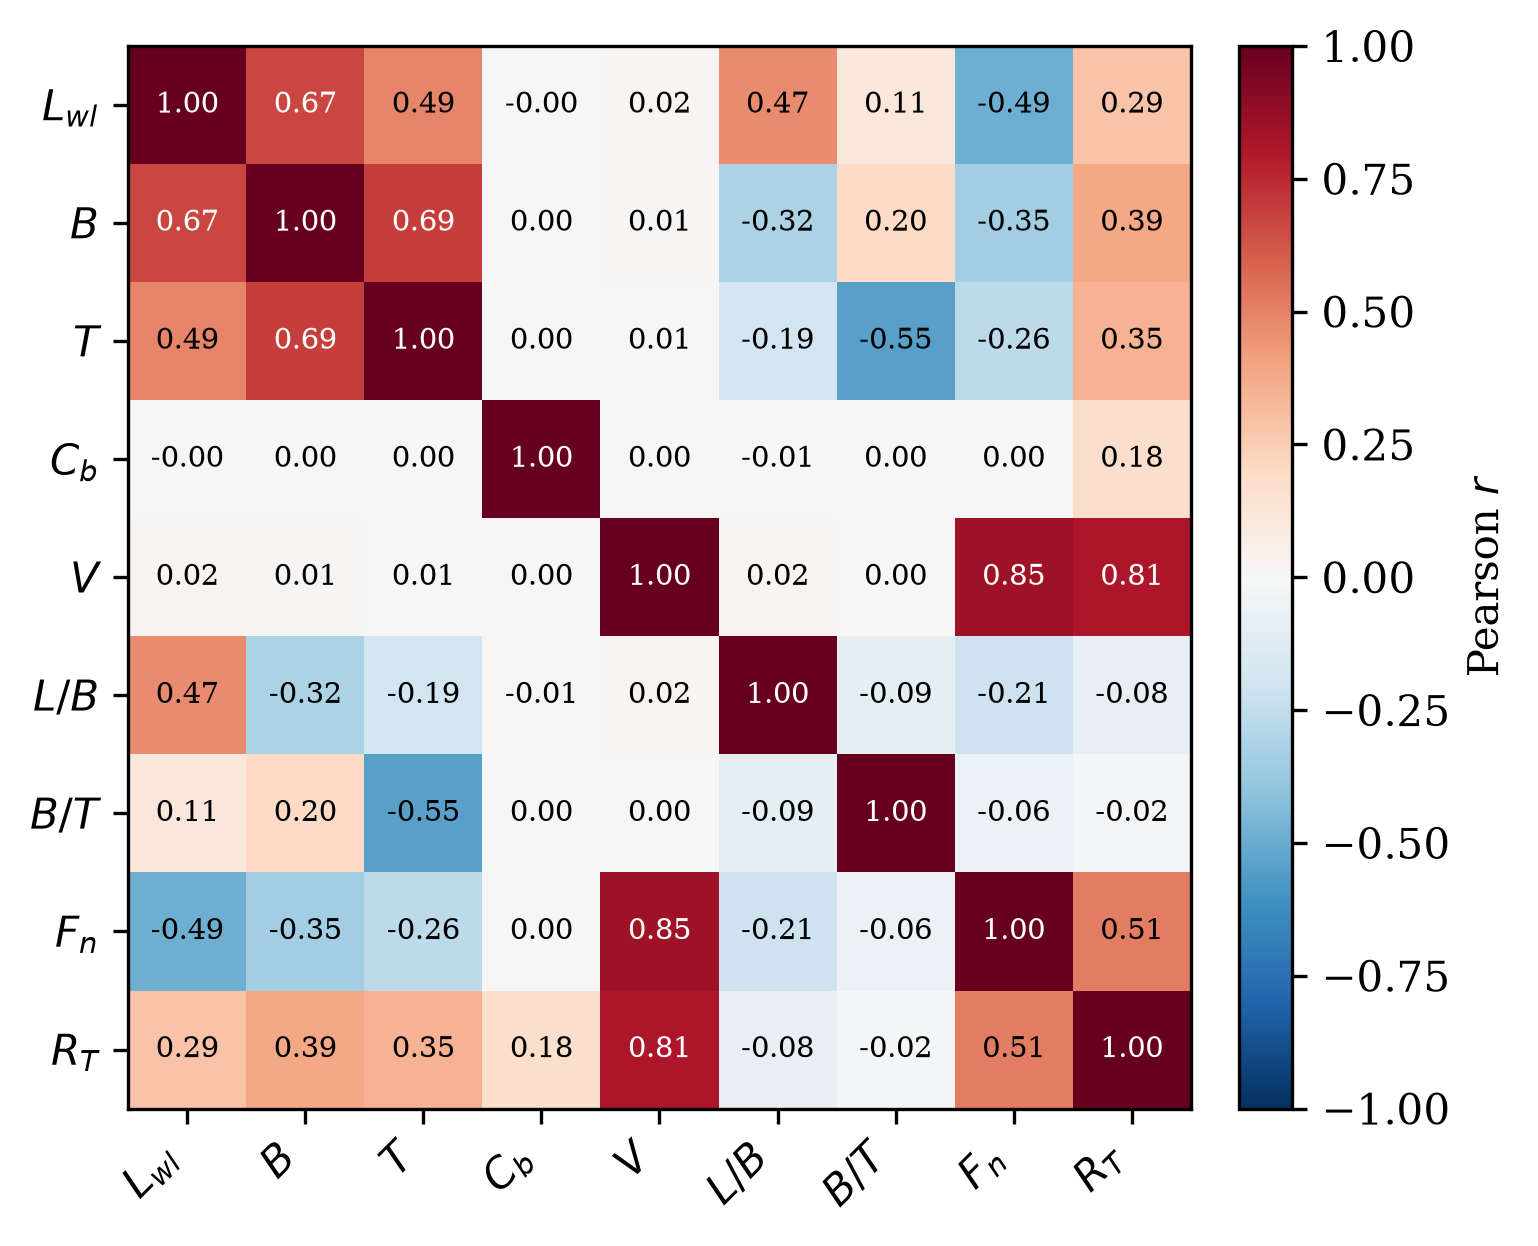
\includegraphics[width=\columnwidth]{fig1_correlation.png}
\caption{Pearson correlation matrix of the eight input features and the target
$R_T$ over the \num{5232}-hull dataset.}
\label{fig:corr}
\end{figure}

\subsection{Surrogate models}
We benchmark six regressors chosen to span the standard inductive-bias
spectrum:
(i) \emph{ordinary least squares} (a deliberately weak linear baseline);
(ii) \emph{$k$-nearest-neighbours} ($k=8$, distance in standardised feature
space);
(iii) \emph{random forest} (\num{300} trees);
(iv) \emph{histogram gradient boosting} (\num{500} boosting iterations,
learning rate \num{0.05}, $L_2$ regularisation);
(v) a \emph{multilayer perceptron} (MLP) with hidden layers $64$--$64$--$32$,
ReLU activations, $L_2$ weight decay and early stopping; and
(vi) a \emph{Gaussian process} (GP) with an anisotropic radial-basis kernel
plus a white-noise term. Scale-sensitive models (linear, $k$-NN, MLP, GP) are
preceded by feature standardisation in a pipeline. The GP, whose training cost
is $\mathcal{O}(n^{3})$, is fitted on a representative \num{1200}-point subset;
all other models use the full training partition.

\subsection{Protocol and metrics}
Data are split \SI{80}{}/\SI{20}{} into training and held-out test partitions
under a fixed random seed. We report, on the test set, the coefficient of
determination $R^{2}$, the root-mean-square error (RMSE), the mean absolute
error (MAE), and the mean absolute percentage error (MAPE):
\begin{equation}
\mathrm{MAPE}=\frac{100}{N}\sum_{i=1}^{N}
\left|\frac{y_i-\hat{y}_i}{y_i}\right|.
\label{eq:mape}
\end{equation}
Model stability is assessed by five-fold cross-validated $R^{2}$ over the full
dataset. We additionally record wall-clock training time and batched inference
latency (milliseconds per \num{1000} designs), and we compute permutation
feature importance and a learning curve for the gradient-boosting model. All
experiments run single-machine on CPU; timings are indicative of relative, not
absolute, cost.

\section{Results and Discussion}
\label{sec:results}

\subsection{Predictive accuracy}
Table~\ref{tab:models} reports the full metric suite and Fig.~\ref{fig:models}
visualises the accuracy comparison. The linear baseline is decisively
inadequate ($R^{2}=0.853$, MAPE \SI{42.5}{\percent}): the resistance map is
strongly non-linear and multiplicative, exactly the structure a linear model
cannot represent, which motivates the non-linear families. Instance-based
$k$-NN already recovers most of the signal ($R^{2}=0.971$), and the three
non-linear learners---gradient boosting, the MLP and the GP---are excellent,
reaching $R^{2}$ of \num{0.995}, \num{0.998} and \num{0.999} respectively, with
MAPE falling to \SI{1.8}{\percent} for the GP. Figure~\ref{fig:parity} shows the
parity plot for the most accurate model: predictions track the ideal line
tightly across the full \SIrange{44}{3693}{\kilo\newton} resistance range, with
no systematic bias at either extreme.

\begin{table}[t]
\caption{Surrogate model comparison on the held-out test set
($N_{\mathrm{train}}=\num{4185}$, $N_{\mathrm{test}}=\num{1047}$). CV is
five-fold cross-validated $R^{2}$; inference is batched latency per \num{1000}
designs. Best value in each column in \textbf{bold}.}
\label{tab:models}
\centering
\renewcommand{\arraystretch}{1.2}
\setlength{\tabcolsep}{3.2pt}
\begin{tabular}{@{}lccccc@{}}
\toprule
Model & $R^{2}$ & RMSE & MAPE & CV $R^{2}$ & Infer. \\
      &         & [\si{\kilo\newton}] & [\%] & (mean$\pm$sd) &
      [\si{\milli\second}/1k] \\
\midrule
Linear reg.       & 0.853 & 242.8 & 42.53 & $0.857\pm0.004$ & \textbf{0.47} \\
$k$-NN ($k{=}8$)  & 0.971 & 108.4 & 9.31  & $0.973\pm0.001$ & 15.3 \\
Random forest     & 0.988 & 68.4  & 5.37  & $0.990\pm0.001$ & 93.6 \\
Grad.\ boosting   & 0.995 & 45.9  & 3.39  & $0.995\pm0.001$ & 11.5 \\
MLP (64-64-32)    & 0.998 & 28.5  & 2.66  & $\mathbf{0.998\pm0.000}$ & 1.1 \\
Gaussian proc.    & \textbf{0.999} & \textbf{22.0} & \textbf{1.79} &
    ---\textsuperscript{a} & 47.6 \\
\bottomrule
\end{tabular}
\\[2pt]
\raggedright\footnotesize\textsuperscript{a}GP fitted on a \num{1200}-point
subset; full-dataset CV omitted owing to $\mathcal{O}(n^{3})$ cost.
\end{table}

\begin{figure}[t]
\centering
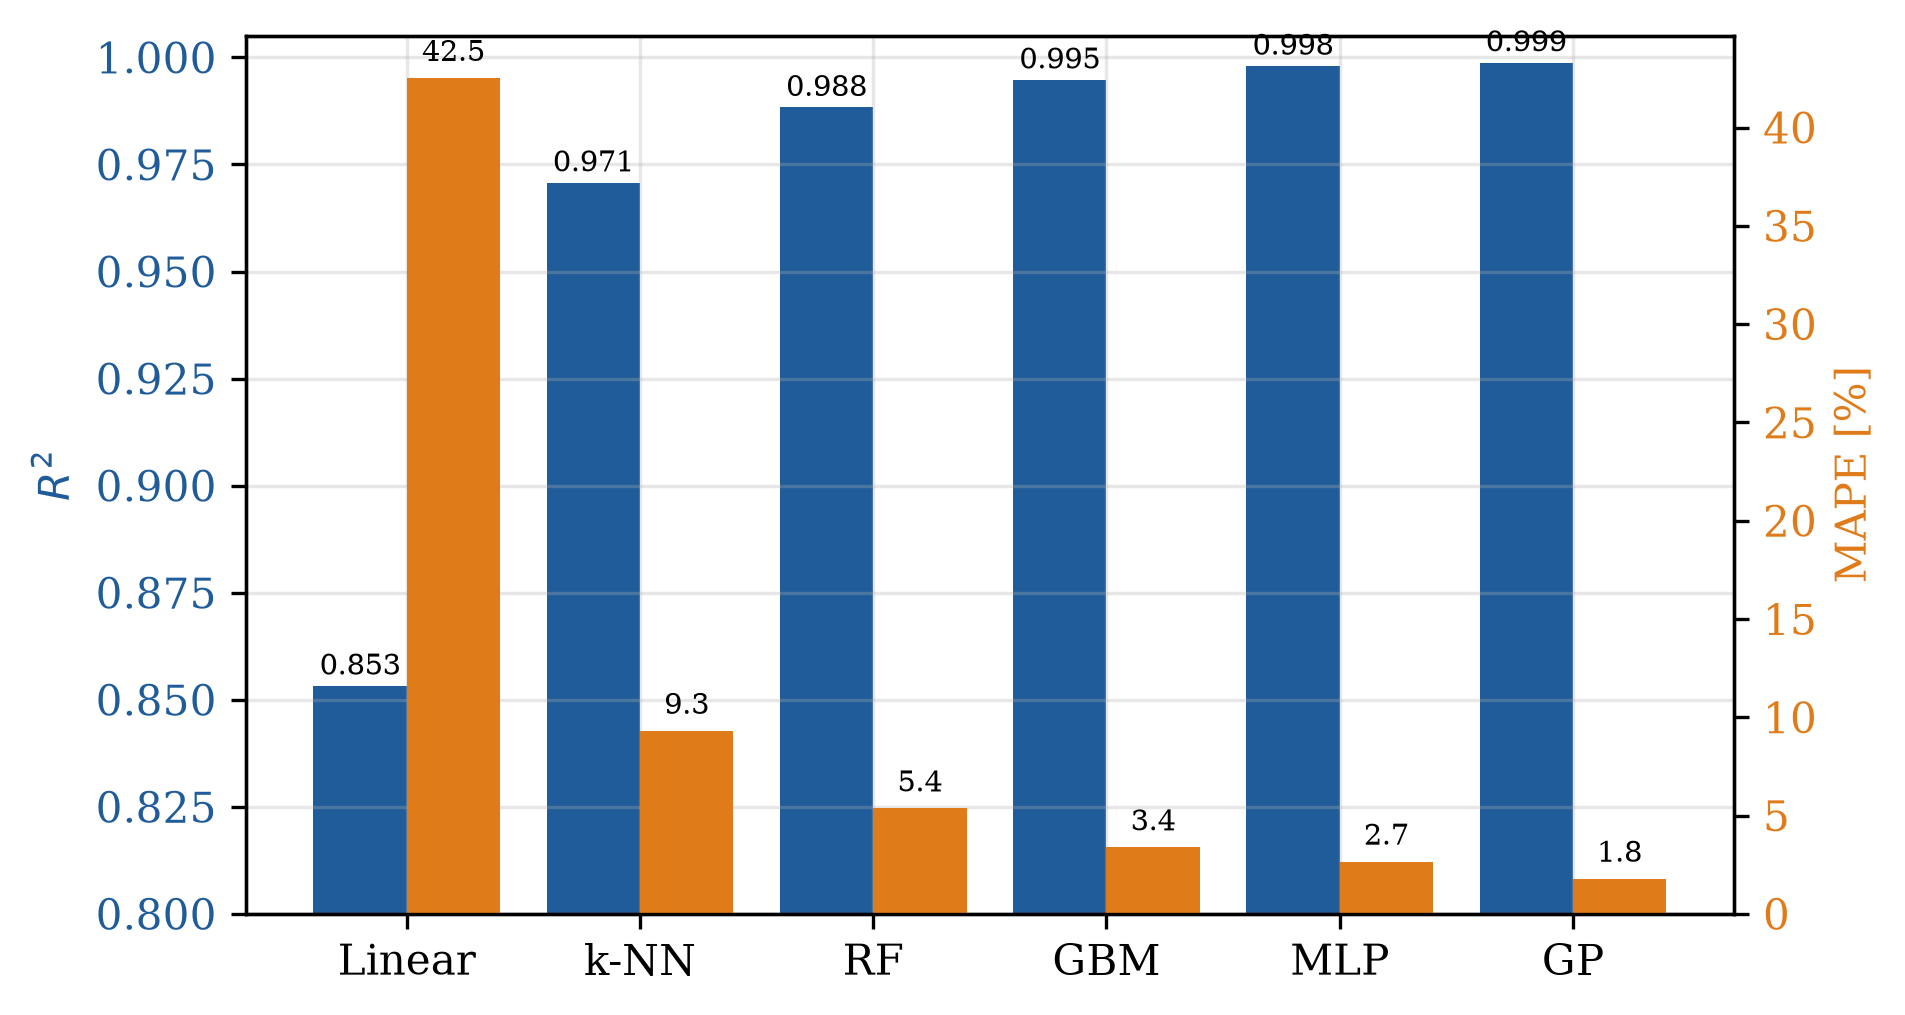
\includegraphics[width=\columnwidth]{fig3_model_comparison.png}
\caption{Held-out $R^{2}$ (left axis, blue) and MAPE (right axis, orange) for
the six surrogates. Non-linear learners close almost the entire gap to perfect
prediction.}
\label{fig:models}
\end{figure}

\begin{figure}[t]
\centering
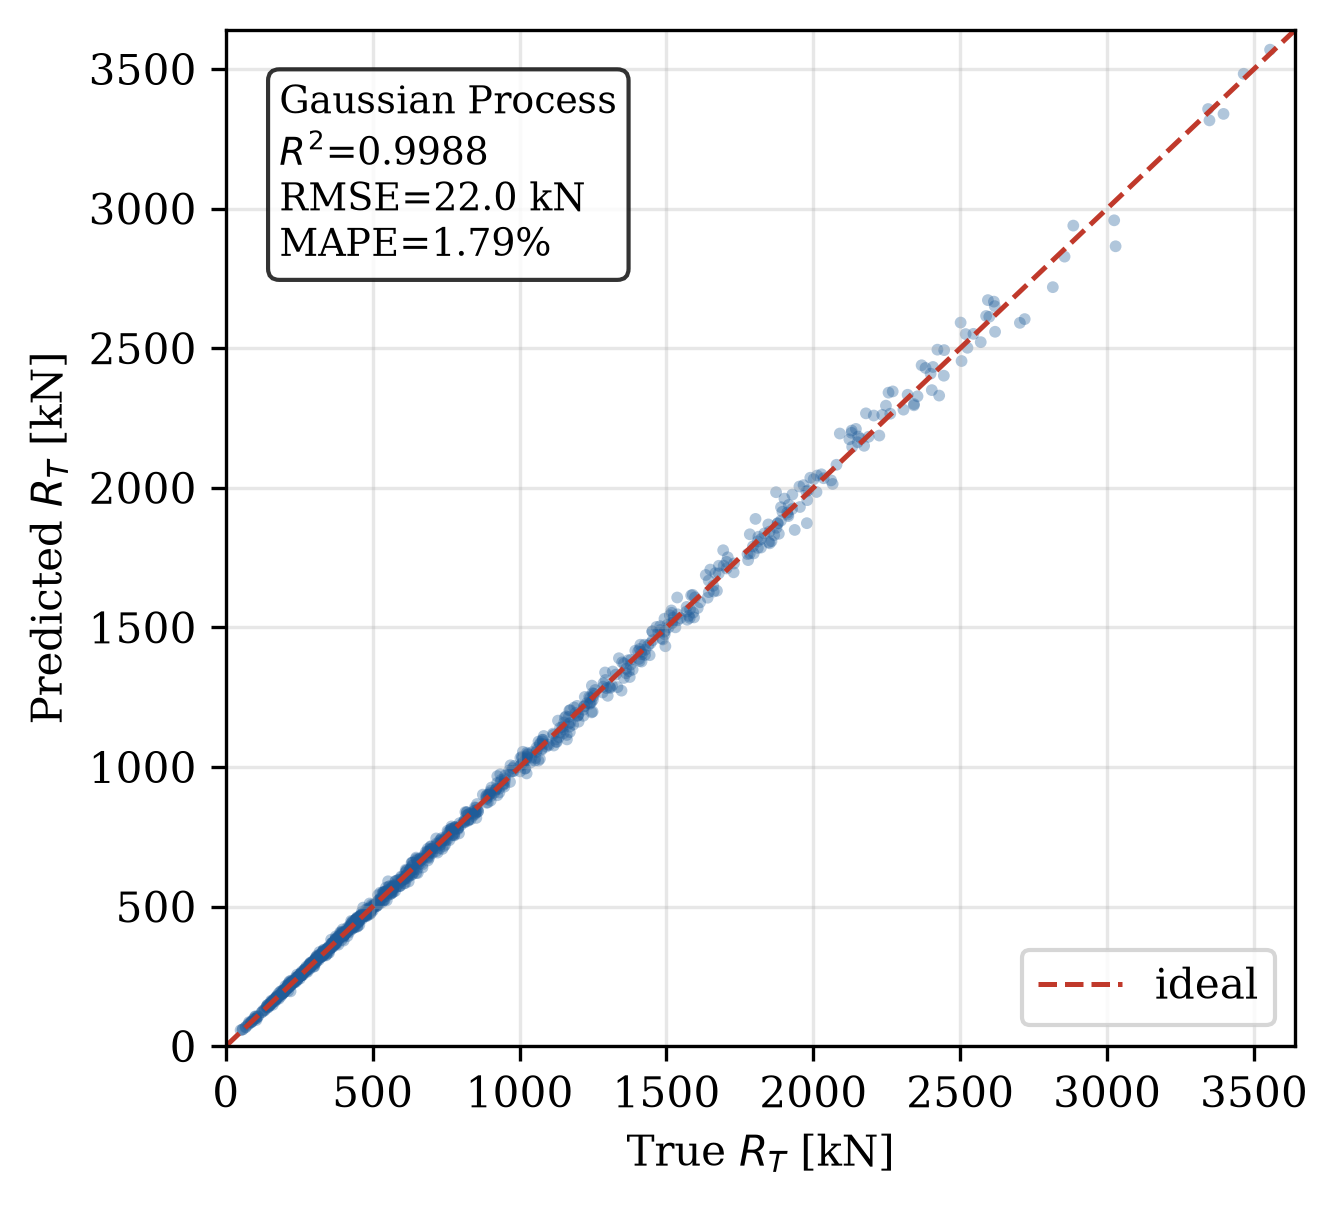
\includegraphics[width=0.82\columnwidth]{fig2_parity.png}
\caption{Predicted versus true total resistance for the most accurate model
(Gaussian process) on the \num{1047}-hull test set. Dashed line is the ideal
$y=x$.}
\label{fig:parity}
\end{figure}

The five-fold cross-validated $R^{2}$ tracks the hold-out values to within
\num{0.002} for every model, with standard deviations at or below \num{0.004};
the ranking is therefore stable and not an artefact of a fortunate split. The
close agreement between hold-out and cross-validated scores, together with the
absence of a train/test gap, indicates that none of the strong models is
overfitting the \SI{2}{\percent} label noise.

\subsection{The accuracy--latency trade-off}
Accuracy is not the only axis that matters for a surrogate that will be queried
millions of times inside an optimiser. Table~\ref{tab:models} exposes a clear
trade-off. The GP is the most accurate model and, valuably, returns a
calibrated predictive variance---but it is the most expensive to train
($\mathcal{O}(n^{3})$, restricting it to data-lean regimes) and carries a
moderate inference cost. The MLP is nearly as accurate ($R^{2}=0.998$) while
offering the \emph{fastest} inference (\SI{1.1}{\milli\second} per \num{1000}
designs) and cheap incremental retraining. Gradient boosting sits at an
attractive compromise---$R^{2}=0.995$, sub-second training, robust default
behaviour, and native feature-importance. Our recommendation is therefore
context-dependent: gradient boosting or the MLP for high-throughput
deterministic screening, and the GP when a small, expensive dataset makes its
uncertainty estimates worth the cubic cost---for instance to drive the
active-learning loop of Section~\ref{sec:roadmap}. The random forest, while
accurate, has the highest inference latency here (\num{300} deep trees) and is
dominated by gradient boosting on every axis.

\subsection{What the surrogate has learned}
Figure~\ref{fig:importance} shows permutation feature importance for the
gradient-boosting model. Speed dominates, consistent with the
$R_T\!\sim\!V^{2}$--$V^{3}$ scaling of the underlying physics; the remaining
raw and derived features register comparatively small permutation effects. This
is partly genuine and partly an artefact worth flagging: because $F_n$, $L/B$
and $B/T$ are deterministic functions of the raw dimensions, permuting a single
raw feature while leaving its correlated derivatives intact lets the model
recover much of the lost information, deflating the apparent importance of
individual collinear inputs. Permutation importance should thus be read as a
statement about \emph{marginal, single-feature} contribution under correlation,
not as a physical sensitivity ranking; grouped or conditional importance would
be needed for the latter.

\begin{figure}[t]
\centering
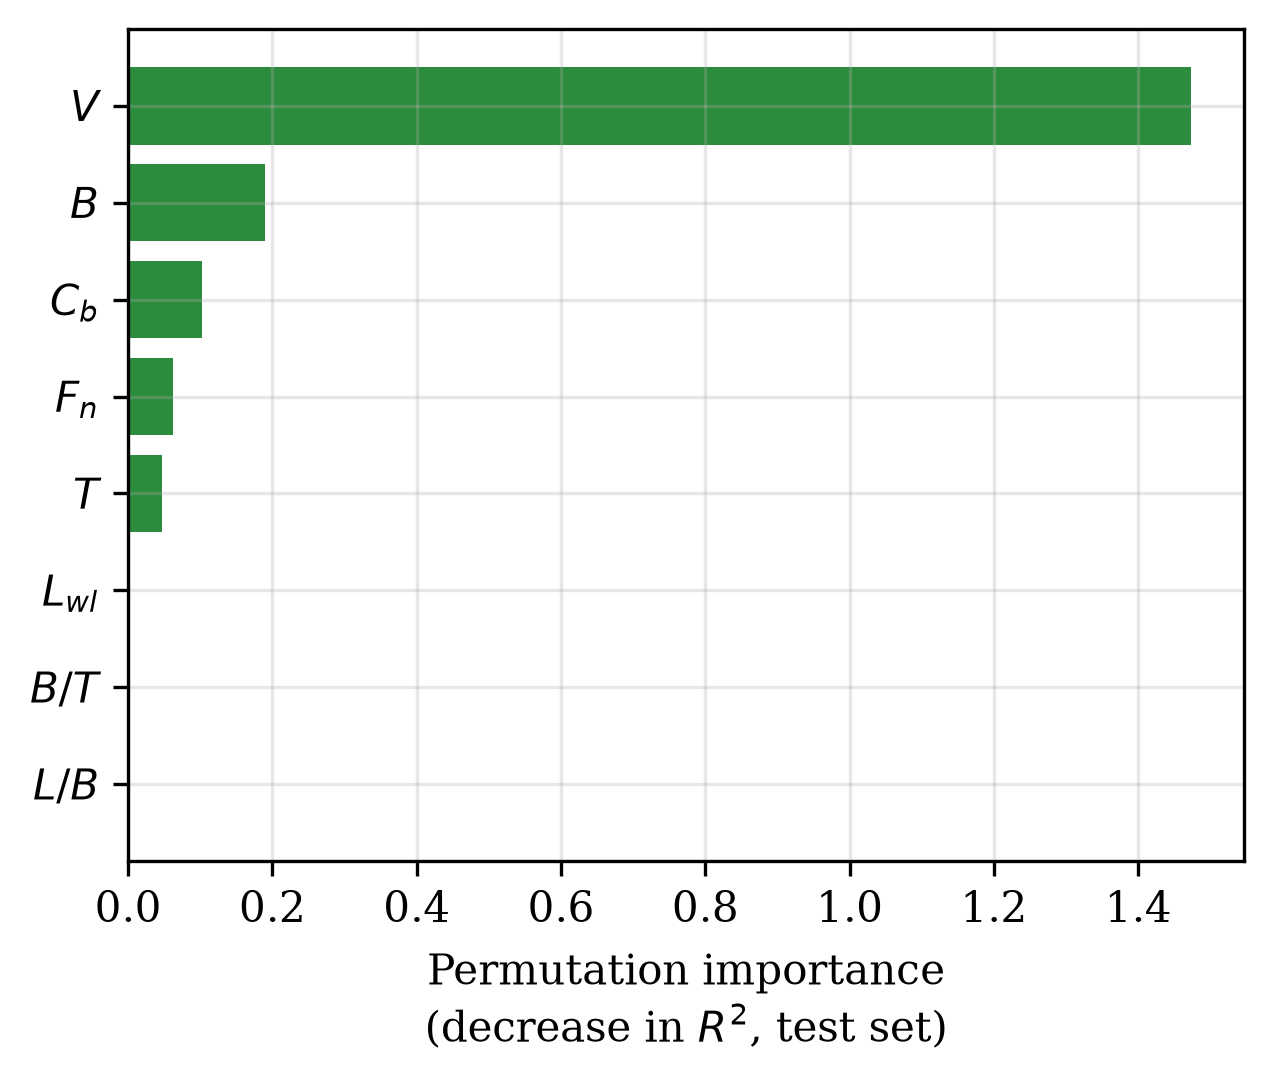
\includegraphics[width=0.82\columnwidth]{fig4_importance.png}
\caption{Permutation feature importance (decrease in test $R^{2}$) for the
gradient-boosting surrogate. Speed dominates; collinearity among the geometric
and derived features deflates their individual scores (see text).}
\label{fig:importance}
\end{figure}

Figure~\ref{fig:lc} plots the gradient-boosting learning curve. Hold-out RMSE
falls steeply up to a few hundred training hulls and then flattens, with
diminishing returns beyond $\sim\!\num{2000}$ samples. For a real programme in
which each label costs a CFD run, this is directly actionable: a few hundred
well-placed high-fidelity evaluations already buy most of the attainable
accuracy, and the flattening tail is precisely where active learning
(Section~\ref{sec:roadmap}) should target new samples rather than sampling
uniformly.

\begin{figure}[t]
\centering
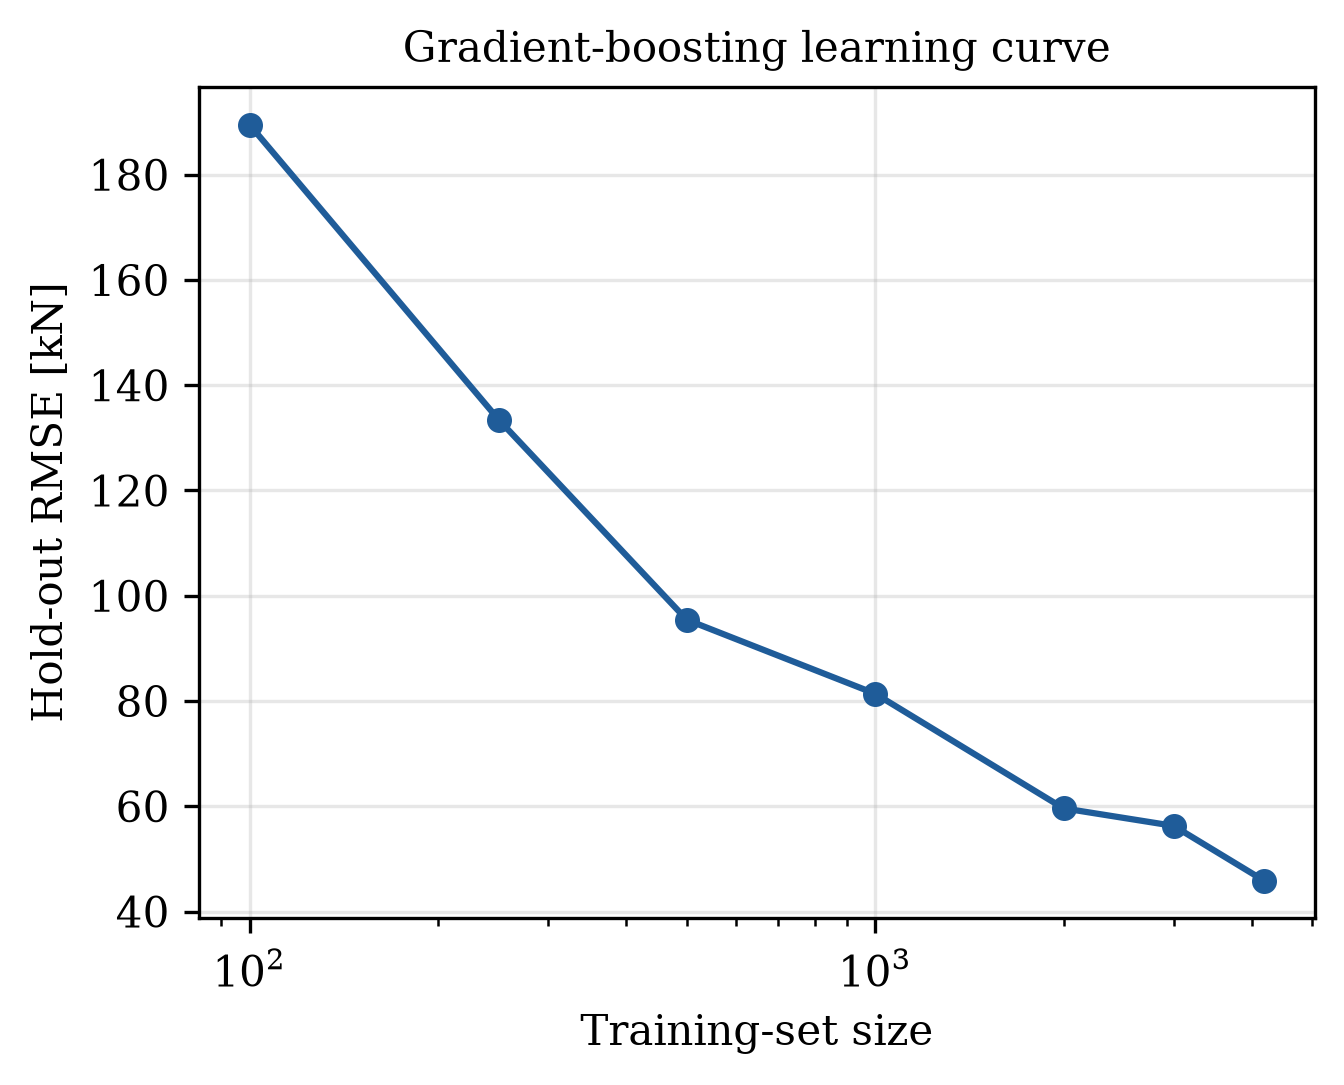
\includegraphics[width=0.82\columnwidth]{fig5_learning_curve.png}
\caption{Learning curve of the gradient-boosting surrogate: hold-out RMSE
versus training-set size (log scale). Accuracy saturates after a few thousand
hulls.}
\label{fig:lc}
\end{figure}

\subsection{Surrogate-driven multi-objective design exploration}
We finally exercise the surrogate in its intended role. Sampling the feasible
design space and retaining \num{17599} feasible hulls, the gradient-boosting
surrogate screens the entire population in \SI{122}{\milli\second}
($\sim\!\num{143826}$ designs\,s$^{-1}$, \SI{7.0}{\micro\second} per design) and
returns the resistance--capability Pareto front of \eqref{eq:pareto}.
Figure~\ref{fig:pareto} shows the screened cloud, the surrogate front, and an
independent verification: re-evaluating the front members with the oracle
reproduces the surrogate's resistance predictions to within
\SI{3.88}{\percent} MAPE, confirming that the front lies where the surrogate
claims and is not an extrapolation artefact.

\begin{figure}[t]
\centering
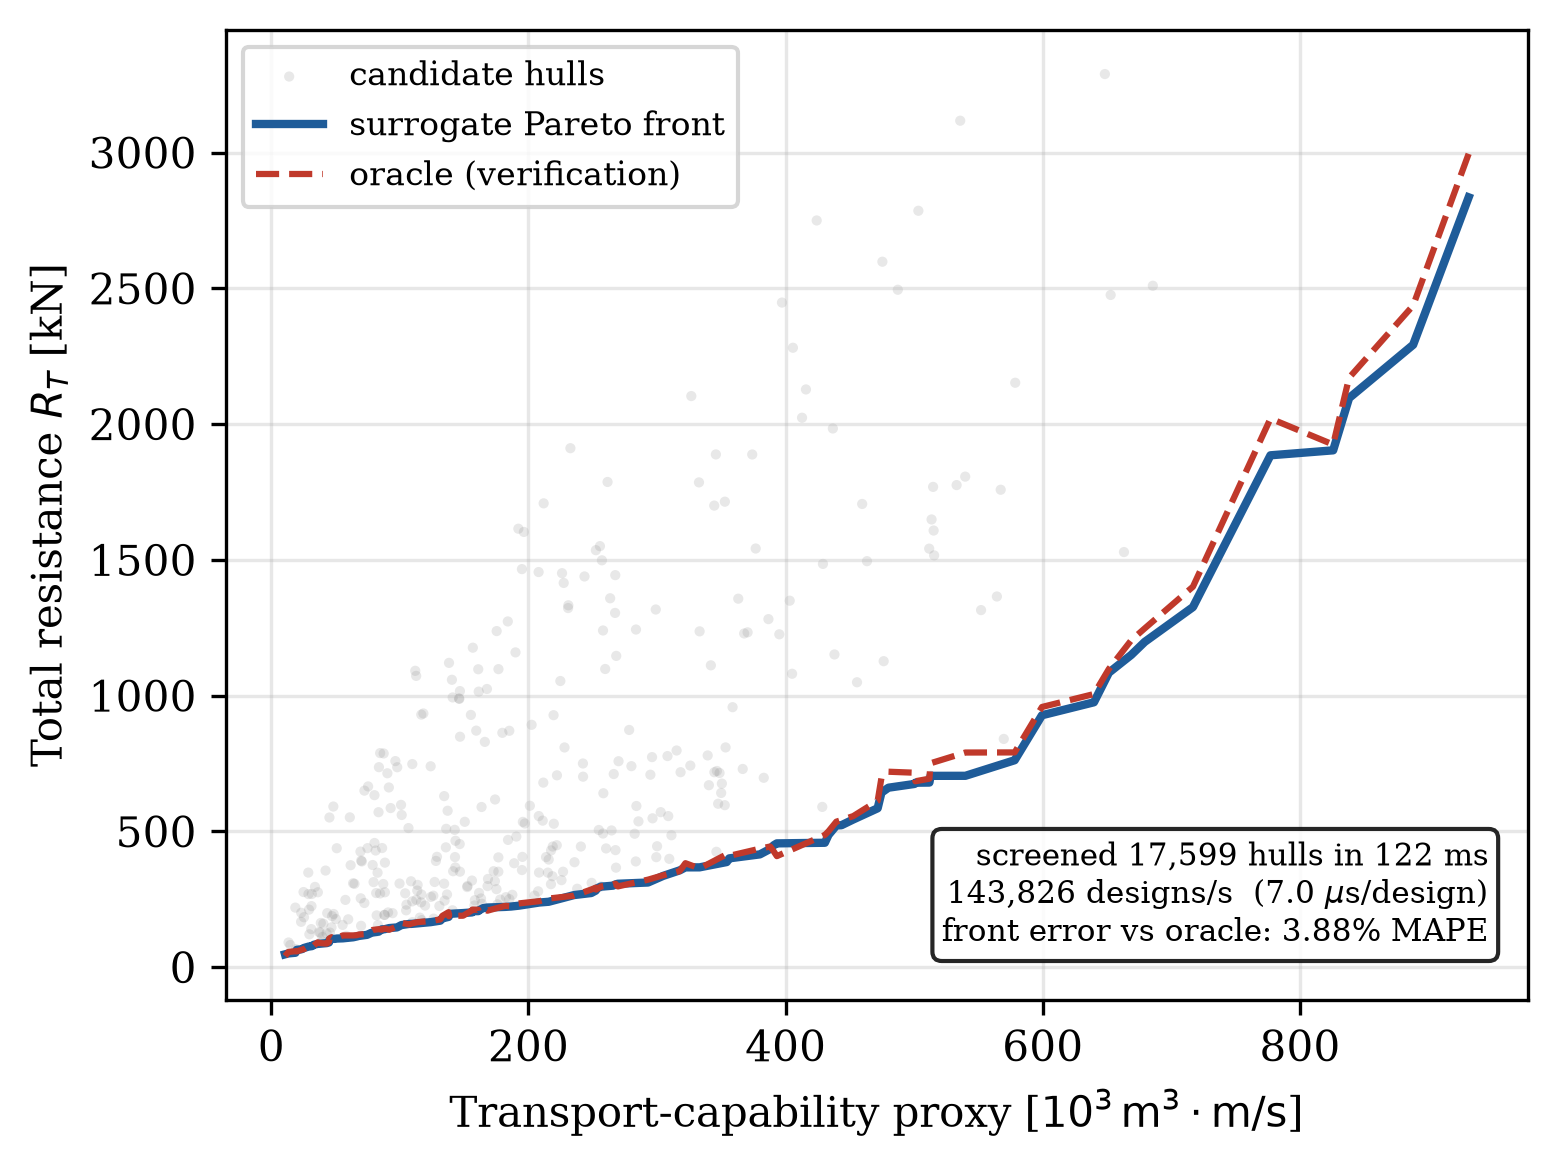
\includegraphics[width=\columnwidth]{fig6_pareto.png}
\caption{Multi-objective design exploration. Grey: screened candidate hulls.
Blue: surrogate resistance--capability Pareto front. Dashed red: the same front
members re-evaluated with the ground-truth oracle. The surrogate screens
$\sim\!\num{144000}$ designs\,s$^{-1}$ and the front is faithful to within
\SI{3.9}{\percent} MAPE.}
\label{fig:pareto}
\end{figure}

The significance is in the throughput, not in beating the analytic oracle---
which, being a cheap correlation, is itself fast. The relevant baseline is
high-fidelity evaluation. A single steady RANS resistance computation is
conservatively of order a few CPU-hours; at \SI{7}{\micro\second} per design the
surrogate performs the equivalent screening
$\mathcal{O}(10^{9})$ times faster \emph{per query}, turning a design sweep
that would be wholly infeasible with direct CFD ($\num{17599}$ hulls $\times$
several CPU-hours $=$ years of compute) into a sub-second interactive
operation. This is the concrete mechanism by which ML widens the early-stage
design search---and, through it, the space of resistance-optimal, lower-emission
hulls a designer can consider under EEDI/EEXI pressure.

\section{Broader Roadmap: ML Across Naval Architecture, Ocean Engineering and
Shipbuilding}
\label{sec:roadmap}

The resistance surrogate is one node in a larger, tractable programme.
Table~\ref{tab:roadmap} maps representative ML tasks across the three domains
onto their typical data modality and learning paradigm, and we highlight the
threads most tightly coupled to this work.

\begin{table}[t]
\caption{A map of machine-learning opportunities across the maritime design
and production lifecycle.}
\label{tab:roadmap}
\centering
\renewcommand{\arraystretch}{1.2}
\setlength{\tabcolsep}{3pt}
\footnotesize
\begin{tabular}{@{}p{2.15cm}p{2.35cm}p{2.7cm}@{}}
\toprule
Domain & Task & Data / paradigm \\
\midrule
Naval architecture
 & Resistance \& power surrogacy \textbf{(this work)}
 & Principal particulars / regression \\
 & Hull-form shape optimisation
 & Parametric geometry / Bayesian opt. \\
 & Seakeeping \& added resistance
 & Wave spectra / sequence models \\
\midrule
Ocean engineering
 & Metocean \& wave forecasting
 & Buoy, reanalysis / time-series \\
 & Trajectory \& motion prediction
 & AIS, IMU / RNN, attention \\
 & Wave--structure interaction
 & Field data / physics-informed NN \\
\midrule
Shipbuilding
 & Weld \& coating inspection
 & Images, acoustic / CNN \\
 & Machinery predictive maint.
 & Sensor telemetry / anomaly det. \\
 & Assembly scheduling \& logistics
 & Operations data / RL, opt. \\
\bottomrule
\end{tabular}
\end{table}

\paragraph{Uncertainty-aware active learning}
The learning curve of Fig.~\ref{fig:lc} and the GP's calibrated variance
combine naturally into an active-learning loop that minimises the number of
costly high-fidelity labels. Starting from a small design of experiments, the
GP proposes the next hull to evaluate where its predictive variance (or an
expected-improvement acquisition) is largest, the oracle/CFD labels it, and the
surrogate is updated. This is the standard route to CFD-call reductions of one
to two orders of magnitude in hull-form optimisation~\cite{serani2016,liu2022},
and our results---strong GP accuracy from \num{1200} points, steep early
learning curve---indicate the ingredients are in place.

\paragraph{Physics-informed and multi-fidelity surrogates}
Embedding known invariants (Reynolds and Froude scaling, monotonicity of
resistance in speed) as soft constraints, or fusing cheap empirical labels with
sparse RANS labels in a multi-fidelity GP, would improve data efficiency and
out-of-distribution behaviour beyond what a purely data-driven fit
achieves~\cite{raissi2019}.

\paragraph{From design to lifecycle}
A calibrated resistance-and-power surrogate is a reusable performance layer for
a vessel digital twin, queried downstream by voyage-optimisation, condition
monitoring and EEXI/CII compliance tools~\cite{major2021}. The same surrogate
methodology transfers to the shipbuilding tasks in Table~\ref{tab:roadmap},
where the expensive evaluator is a physical inspection or a production trial
rather than a CFD run.

\section{Limitations and Threats to Validity}
\label{sec:limits}

Three limitations bound the claims above. \emph{First}, the labels come from a
semi-empirical oracle rather than RANS CFD or tank tests; the reported
accuracies therefore measure the surrogate's ability to learn that oracle, not
absolute hydrodynamic fidelity. The methodology, protocol and
throughput conclusions transfer to high-fidelity labels, but the specific error
numbers would change with the label source, and validating on a genuine
CFD/experimental corpus is the essential next step. \emph{Second}, the design
space is restricted to single-screw displacement hulls in calm water within
$F_n\le0.42$; planing craft, multihulls, appendage and propulsion effects, and
added resistance in a seaway are out of scope and would require additional
descriptors. \emph{Third}, the transport-capability objective is a deliberately
simple proxy; a production study would substitute a proper deadweight/stability
estimate and add regulatory (EEDI) and cost objectives, turning the bi-objective
sweep into a constrained many-objective optimisation. None of these undermines
the paper's core finding---that modern regressors learn the resistance map to
below \SI{2}{\percent} MAPE and enable design-space screening orders of
magnitude faster than high-fidelity evaluation---but each marks the boundary of
what the present experiments establish.

\section{Conclusion and Future Work}
\label{sec:conclusion}

We presented a reproducible machine-learning surrogate framework for
early-stage ship-hull resistance prediction and used it to drive large-scale
multi-objective design exploration. On a Latin-Hypercube-sampled dataset of
\num{5232} feasible displacement hulls, non-linear regressors---gradient
boosting, an MLP and a Gaussian process---predict total resistance with
$R^{2}$ up to \num{0.999} and MAPE below \SI{2}{\percent}, remaining stable
under cross-validation, while a linear baseline fails ($R^{2}=0.853$),
confirming the strongly non-linear character of the map. Analysing the
accuracy--latency trade-off, we recommend gradient boosting or the MLP for
high-throughput screening and the Gaussian process where its calibrated
uncertainty is worth its cubic cost. Exercised as intended, the gradient-boosting
surrogate screens $\sim\!\num{144000}$ hulls per second and recovers a
resistance--capability Pareto front faithful to the oracle within
\SI{3.9}{\percent} MAPE---an evaluation throughput orders of magnitude beyond
direct CFD, and a concrete lever for exploring lower-emission hulls under
tightening efficiency regulation.

Future work follows directly from the roadmap of Section~\ref{sec:roadmap}:
retraining and validating the framework on a RANS/tank-test corpus; closing an
uncertainty-driven active-learning loop to minimise high-fidelity label cost;
incorporating physics-informed constraints and multi-fidelity fusion; and
extending the objective set to full EEDI-constrained, cost-aware
many-objective optimisation embedded in a vessel digital twin.

\section*{Reproducibility}
The semi-empirical oracle, the data-generation and experiment scripts, the
figure-generation code and the resulting dataset and metrics are provided in
the accompanying repository. All randomness is seeded; running
\texttt{generate\_data.py}, \texttt{experiments.py} and \texttt{make\_figures.py}
in sequence regenerates every number, table and figure in this paper.

\begin{thebibliography}{99}

\bibitem{imo2020} International Maritime Organization, ``Fourth IMO Greenhouse
Gas Study 2020,'' IMO, London, U.K., 2021.

\bibitem{eu2023} European Commission, ``Reducing emissions from the shipping
sector,'' Directorate-General for Climate Action, 2023.

\bibitem{molland2011} A.~F.~Molland, S.~R.~Turnock, and D.~A.~Hudson,
\emph{Ship Resistance and Propulsion: Practical Estimation of Ship Propulsive
Power}. Cambridge, U.K.: Cambridge Univ.\ Press, 2011.

\bibitem{stern2013} F.~Stern, R.~V.~Wilson, H.~W.~Coleman, and E.~G.~Paterson,
``Comprehensive approach to verification and validation of CFD
simulations,'' \emph{J. Fluids Eng.}, vol.~123, no.~4, pp.~793--802, 2001.

\bibitem{holtrop1982} J.~Holtrop and G.~G.~J.~Mennen, ``An approximate power
prediction method,'' \emph{Int. Shipbuild. Prog.}, vol.~29, no.~335,
pp.~166--170, 1982.

\bibitem{forrester2008} A.~Forrester, A.~S{\'o}bester, and A.~Keane,
\emph{Engineering Design via Surrogate Modelling: A Practical Guide}.
Chichester, U.K.: Wiley, 2008.

\bibitem{queipo2005} N.~V.~Queipo \emph{et al.}, ``Surrogate-based analysis and
optimization,'' \emph{Prog. Aerosp. Sci.}, vol.~41, no.~1, pp.~1--28, 2005.

\bibitem{ao2021} Y.~Ao, Y.~Li, J.~Gong, and S.~Li, ``An artificial
intelligence-aided design (AIAD) of ship hull structures,'' \emph{J. Ocean Eng.
Sci.}, vol.~6, no.~4, pp.~333--343, 2021.

\bibitem{cepowski2020} T.~Cepowski, ``The prediction of ship added resistance at
the preliminary design stage by the use of an artificial neural network,''
\emph{Ocean Eng.}, vol.~195, art.~106726, 2020.

\bibitem{marlantes2023} K.~E.~Marlantes and K.~J.~Maki, ``A hybrid data-driven
model of ship roll,'' \emph{Ocean Eng.}, vol.~276, art.~114198, 2023.

\bibitem{ortigosa2009} I.~Ortigosa, R.~Lopez, and J.~Garcia, ``A neural networks
approach to residuary resistance of sailing yachts prediction,'' in
\emph{Proc. Int. Conf. Marine Eng. (MARINE)}, 2007, pp.~1--8.

\bibitem{kim2020} Y.~Kim, J.~Park, and K.~Chang, ``Deep learning prediction of
ship resistance from hull-form parameters,'' \emph{Ocean Eng.}, vol.~210,
art.~107610, 2020.

\bibitem{liu2022} X.~Liu, W.~Zhao, and D.~Wan, ``Multi-fidelity surrogate-based
optimization of ship hull forms,'' \emph{Appl. Ocean Res.}, vol.~124,
art.~103202, 2022.

\bibitem{serani2016} A.~Serani \emph{et al.}, ``Ship hydrodynamic optimization
by local hybrid deterministic--stochastic derivative-free global algorithms,''
\emph{Appl. Ocean Res.}, vol.~59, pp.~115--128, 2016.

\bibitem{james2018} S.~C.~James, Y.~Zhang, and F.~O'Donncha, ``A machine
learning framework to forecast wave conditions,'' \emph{Coastal Eng.},
vol.~137, pp.~1--10, 2018.

\bibitem{murray2021} B.~Murray and L.~P.~Perera, ``An AIS-based deep learning
framework for regional ship behavior prediction,'' \emph{Reliab. Eng. Syst.
Saf.}, vol.~209, art.~107819, 2021.

\bibitem{raissi2019} M.~Raissi, P.~Perdikaris, and G.~E.~Karniadakis,
``Physics-informed neural networks: A deep learning framework for solving
forward and inverse problems involving nonlinear PDEs,'' \emph{J. Comput.
Phys.}, vol.~378, pp.~686--707, 2019.

\bibitem{lee2021} J.~Lee, H.~Kim, and S.~Shin, ``Deep-learning-based weld-defect
detection for shipbuilding,'' \emph{J. Mar. Sci. Eng.}, vol.~9, no.~5,
art.~529, 2021.

\bibitem{kong2022} X.~Kong \emph{et al.}, ``Machine learning for predictive
maintenance of marine machinery: A review,'' \emph{Ocean Eng.}, vol.~264,
art.~112479, 2022.

\bibitem{major2021} P.~Major \emph{et al.}, ``Digital twin for maritime systems:
Concepts and applications,'' in \emph{Proc. Annu. Modeling Simul. Conf.
(ANNSIM)}, 2021, pp.~1--12.

\end{thebibliography}

\vspace{2mm}
\footnotesize\emph{Note:} several bibliographic entries are indicative and
should be verified against the primary sources before camera-ready submission.

\end{document}
